% !TEX root = my-thesis.tex
%
\chapter{Implementation}
\label{ch:implementation}

The following chapter provides information about our implementation decisions.
First, we briefly review implementations of related approaches. This is 
followed by a detailed description of our implementation, 
including an overview of the architecture used for training the agent and the interactions between the various components.
The open-source implementation of our approach can be found at \url{https://github.com/LukasBluebaum/Master_Thesis}.

\section{Frameworks}
\label{sec:frameworks}

To begin with, we looked into the implementations of prior works for reinforcement 
learning on knowledge graphs. Most implementations were in Python~\cite{Xiong2017DeePpath,Das2018Minerva, Kaiser2021Reinforcement},
with some exceptions in C++~\cite{Zhang2018Variational} or even C\#~\cite{Shen2018MWalk}.
Comparing the usage of deep learning frameworks in the Python implementations, it was a mix between PyTorch~\cite{Paszke2019Torch} and TensorFlow~\cite{Abadi2015Tensorflow}.
Interestingly, most approaches did not use a specialized reinforcement learning framework but
wrote their implementation from scratch. 

Following CONQUER~\cite{Kaiser2021Reinforcement}, we first implemented a minimal working version using TF-Agents~\cite{Guadarrama2018TFAgents}, 
a reinforcement learning framework that is natively integrated into TensorFlow.
However, we realized the framework is a bit outdated and hard to extend.
Therefore, we looked into other reinforcement learning frameworks like RLlib~\cite{Liang2018rllib} 
and Stable-Baselines3~\cite{Raffin2021Stable}.
In fact, we encountered similar problems, as it would mean a lot of work to extend the frameworks to the appropriate knowledge graph setting for our needs.
Thus, we also decided to write our implementation from scratch using Python and PyTorch, similar 
to most other approaches.

For the extraction and pre-processing of the binary causal questions, we used the NLP frameworks 
NLTK~\cite{BirdKleinLoper2009NLTK} and Stanford CoreNLP~\cite{Manning2014NLP}.
For logging, experiment tracking, and model archival, we used Weights \& Biases~\cite{Biewald2020Wandb}.
Additionally, we used Huggingface Transformers~\cite{Wolf2020Transformers} for one of the baselines in 
our experiments.

\section{Architecture}
\label{sec:architecture}

As described in Section~\ref{sec:frameworks}, we wrote our implementation from scratch without any 
specialized reinforcement learning framework. Still, our implementation is influenced by the 
general structure of frameworks like Stable-Baselines3~\cite{Raffin2021Stable} or 
TF-Agents~\cite{Guadarrama2018TFAgents}.

Figure~\ref{fig:implementation} shows the architecture of our implementation in the form of a UML Class Diagram.
The \textit{EmbeddingProvider} classes are simple wrappers around the embeddings and provide 
methods to retrieve embeddings for entities and relations.\footnote{In our experiments, we used GloVe~\cite{Pennington2014Glove} embeddings since they performed better than BERT embeddings~\cite{Liu2019Roberta}. Therefore, the \textit{BERTEmbeddings} class is just provided for the sake of completeness.} 
These methods are called once by the \textit{KnowledgeGraph} class with lists of entities 
and relations of the current graph.
Note that we kept the implementations of the \textit{EmbeddingProvider} and \textit{KnowledgeGraph} classes more general to allow for the integration 
of graphs with multiple relation types. In the case of CauseNet, all methods dealing with \textit{relations} will 
return the sentence from the metadata for the given entity pair. Moreover, for CauseNet, the 
\textit{KnowledgeGraph} class stores the graph as an adjacency list together with an associative array that 
maps each entity pair to its sentence. Moreover, each entity is assigned an ID. Additionally, it provides methods to retrieve the embedding for a given entity, 
the embedding of the sentence of an entity pair, and the neighbors of an entity. 

The \textit{Environment} class handles the current state of the agent at each time step.
Whenever the \textit{reset} method is called, the environment selects the next question and positions 
the agent on the cause $e_c = e_0$ contained in the question. Afterward, it returns the embeddings for 
the state $[\mathbf{q};\mathbf{e_0}]$ and the action embedding matrix $\mathbf{A_t}$ as described in 
Section~\ref{sec:network}.\footnote{We assume that the embeddings for the question $q$ were precomputed and are part of the question objects.} Similarly, the \textit{step} method receives an action at each time step $t$ and evolves the 
environment accordingly. Next, it returns the embeddings $[\mathbf{q};\mathbf{e_t}]$ and the embedding matrix $\mathbf{A_t}$ together 
with the reward $r_t$ and a boolean value indicating whether the path rollout length $T$ is reached.
As commonly done, we use two \textit{Environment} instances, one for training and one for 
evaluation~\cite{Guadarrama2018TFAgents, Liang2018rllib, Raffin2021Stable}.
The reason is that the behavior in reinforcement learning problems often differs between 
training and inference time. In our case, the behavior changes w.r.t. positive and negative causal questions (Section~\ref{sec:approach-description}) 
and different decoding methods at inference time (Section~\ref{sec:search}).

The \textit{Agent} class consists of the policy network and value network. The value network 
returns a scalar predicting the value of the current state $s_t$, and the policy network returns a
probability distribution over all actions $a_t \in A(s_t)$.
The \textit{Trainer} class does not use the value network if we only use the REINFORCE algorithm.
The \textit{Trainer} class optimizes the \textit{Agent} according to the given parameters.
During each training step, the \textit{Trainer} applies the \textit{Agent} on the \textit{Environment} 
through the \textit{reset} and \textit{step} functions to sample path rollouts. Specifically, 
the \textit{Trainer} provides the output of the \textit{Environment} to the \textit{Agent}, receives 
an action from the \textit{Agent}, and applies it on the Environment via the \textit{step} function.
The path rollouts are stored in the \textit{PathRolloutStorage} until a full batch is accumulated.
Consequently, the \textit{Trainer} performs a gradient step on the \textit{Agent} as described in 
Section~\ref{sec:approach-description}, and the next training iteration starts.
The \textit{Trainer} is an abstract class implemented by the \textit{A2CTrainer} and the
 \textit{REINFORCETrainer}, which run the A2C and REINFORCE algorithms described in 
 Section~\ref{subsec:rl} and Section~\ref{sec:approach-description}.

 Generally, the diagram should only provide a high-level overview. In particular, not all 
 parameters or components are depicted. For example, the computation of rewards and advantages, including the reward shaping 
 and the decoding methods at inference time, are hidden in the \textit{Environment} and \textit{Trainer}
 classes. Moreover, parameters like the supervised ratio $\alpha$ or the supervised batch size are also 
 missing. The exact details can be seen in the code on our repository.

\begin{figure}[htbp]
	\centering
	%\includesvg{figures/implementation2}
	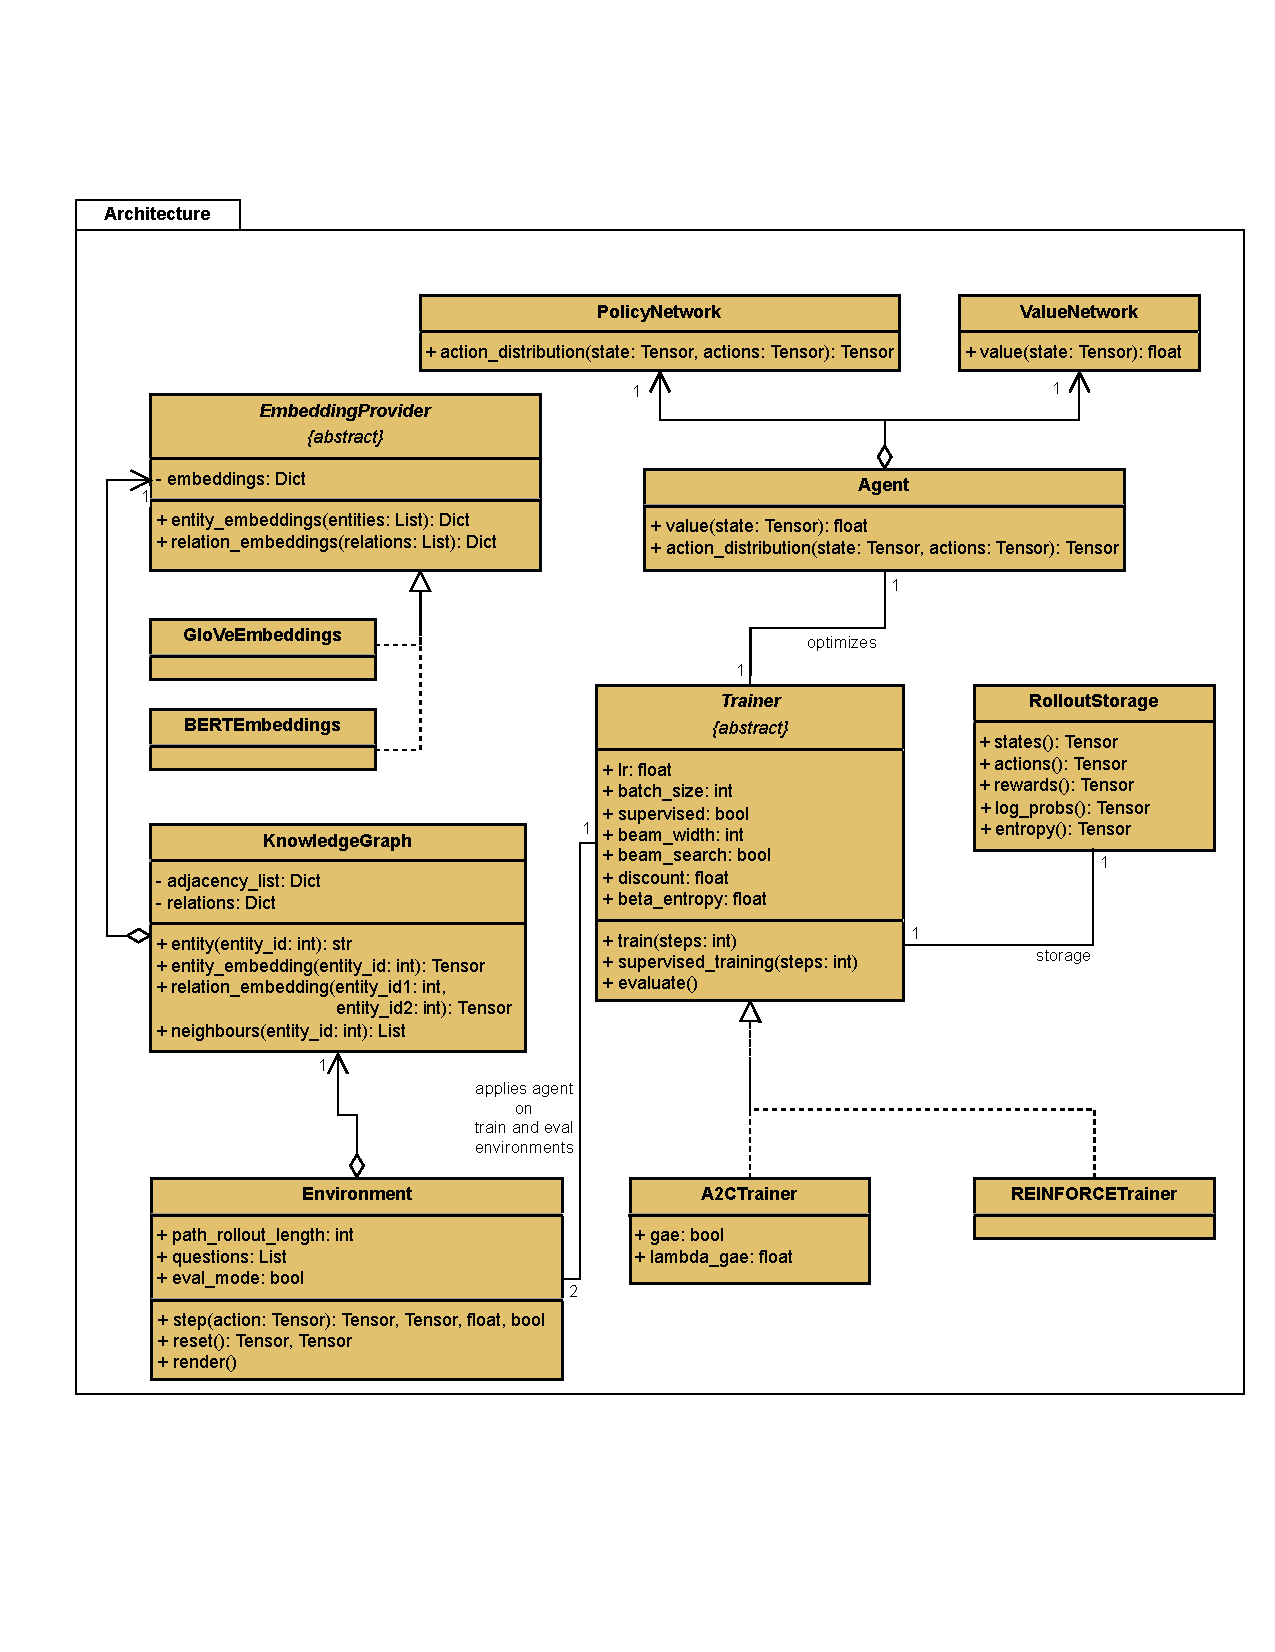
\includegraphics[clip, trim=0cm 4cm 0cm 2cm, width=1.15\textwidth]{figures/implementation}
	\caption{UML-Diagram depicting the architecture of our implementation. It shows the most important 
	classes, including the Trainer, Agent, and Environment, and how they interact with each other. For brevity, not 
	all parameters or methods are shown. Therefore, this figure should only provide a high-level overview. For the complete picture, 
	we provide an open-source implementation at: \\ \url{https://github.com/LukasBluebaum/Master_Thesis}}
	\label{fig:implementation}
  \end{figure}